\subsection{Speed autopilot}\label{subsec:prob1.2}
We started studying the steady state characteristics of the surge speed as a function of propeller shaft velocity. 
\begin{figure}[H]
    \centering
    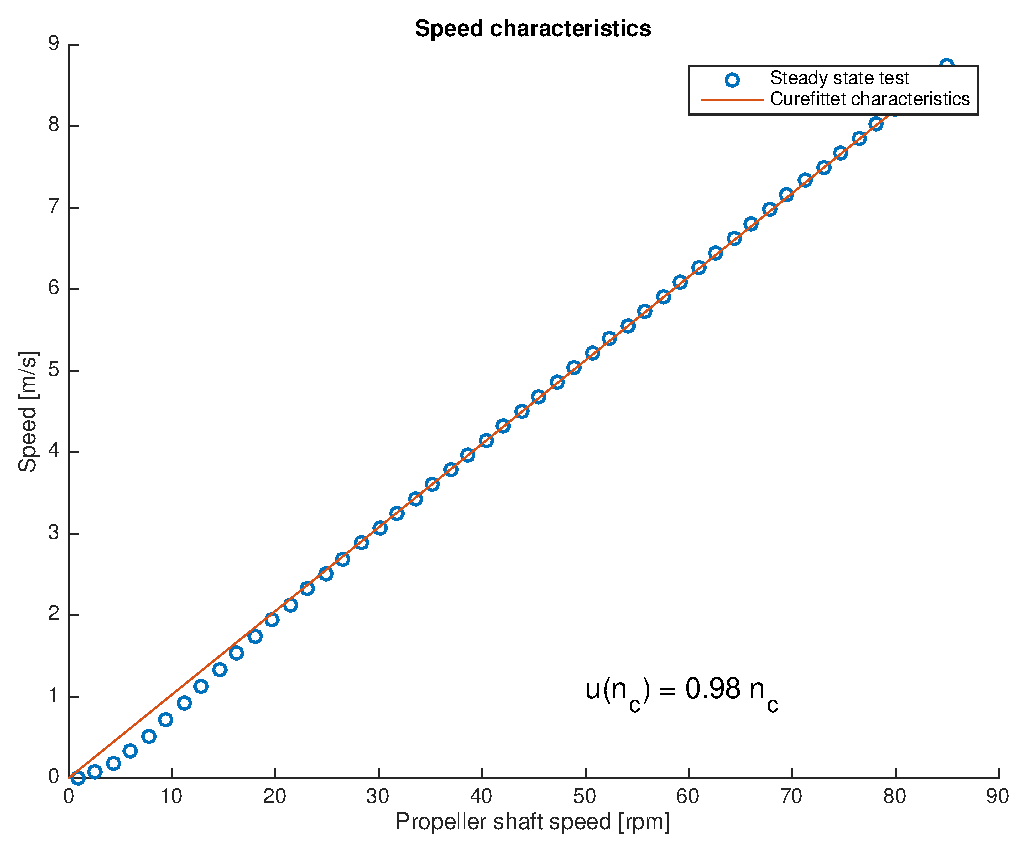
\includegraphics[width=0.9 \textwidth]{task1.8/Speed_characteristics}
    \caption{Speed characteristics}
    \label{fig:1.8-ss}
\end{figure}
As can be seen in figure \ref{fig:1.8-ss}, the characteristics of the ships surge speed is linear. This motivates a first or second order linear surge speed model, where the surge speed is decoupled from the rest of the system. We are assuming $$u>>v$$ which leads to: $$U=u$$ We then try a first order linear model.
\begin{equation}
\frac{u}{n_c}(s) = \frac{K}{1+Ts}
\end{equation}
Which gives us a quite good estimate of the speed dynamics (figure \ref{fig:1.8-speed-model}). Although we have a linear steady state relationship between shaft and surge speed, the time constant varies. This is a sign of a non-linear effect like quadratic damping. 
\begin{figure}[H]
    \centering
    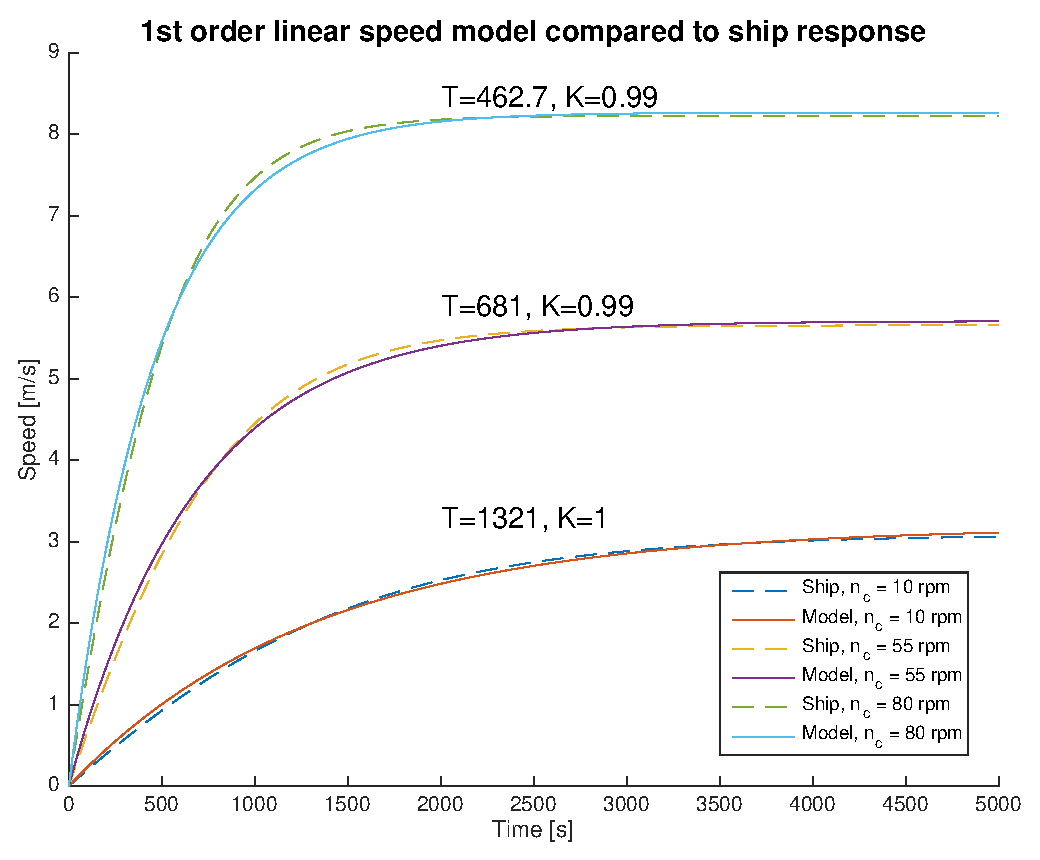
\includegraphics[width=0.9 \textwidth]{task1.8/Task1_8_speed_model}
    \caption{1.order linear speed model}
    \label{fig:1.8-speed-model}
\end{figure}


\begin{figure}[H]
    \centering
    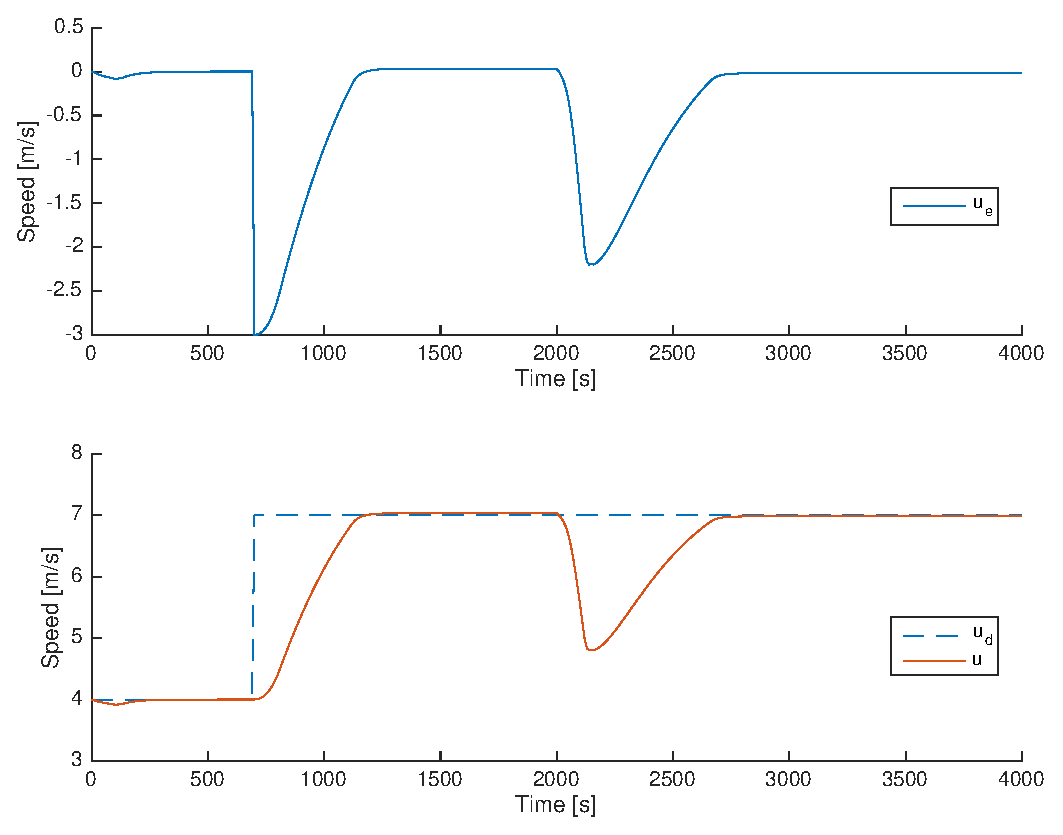
\includegraphics[width=0.9 \textwidth]{task1.8/Task1_8_sim}
    \caption{Speed step response}
    \label{fig:1.8-step}
\end{figure}